\Chapter{ARTICLE: ON HISTORY-AWARE MULTI-ACTIVITY EXPERTISE MODELS}\label{sec:Theme3}

\section{Abstract}

% \begin{abstract}
As software evolves, a developer's contributions will gradually vanish as they are being replaced by other developers' code, slowly eroding the developer's footprint in the software project. Even though this developer's knowledge of the file did not disappear overnight, to outsiders, the developer and her expertise have become invisible. Through an empirical study on 5 years of Linux development history, this paper analyses this phenomenon of expertise erosion by building a 2-dimensional model of developer expertise involving a range of developer activities and involving activity data on more than one release. Using these models, we found that although many Linux maintainers' own coding footprint has regressed over time, their expertise is perpetuated through involvement in other development activities such as patch reviews and committing upstream on behalf of other developers. Considering such activities over time further improves the expertise models.
% \end{abstract}



\section{Introduction}


%Software comprehension is widely accepted to be difficult. Joining a software development team involves a steep learning
%curve. During this period, one has to learn--at the same time--the architecture of a system, its implementation
%rational, the idiosyncrasies of its implementation, its coding standards, the libraries that it uses, etc. etc.
As reported by Damien et al.~\citep{turnover}, employee turnover is a major challenge of information technology organizations. Estimations of the cost of losing an employee amount to between 0.5 and 1.5 times her salary, with the cost of replacing a software engineer in particular exceeding \$100,000~\citep{economist5988}. These costs are not limited to the software engineer's company, but also spread to open source development. In their 2017 Linux kernel report, Corbet et al.~\citep{corbet17} noted that ``well over 85 percent of all kernel development is demonstrably done by developers who are being paid for their work''. In fact, only 8.2\% of all kernel commits were made by volunteer developers. Hence, developer turn-over in companies risks to impact open source development as well!
% ``increasing number of companies are working toward the improvement of the kernel.''
%
% ``It is worth no ng that, even if one assumes that all of the “unknown” contributors are working on their own  me, well over 85 percent of all kernel development is demonstrably done by developers who are being paid for their work.''
%
% ``Interes ngly, the volume of contribu ons from unpaid developers has been in slow decline for many years. It was 14.6 percent in the 2012 version of this report, but is 8.2 percent this  me around. There are many possible reasons for this decline, but, arguably, the most plausible of those is quite simple: kernel developers are in short supply, so anybody who demonstrates an ability to get code into the mainline tends not to have trouble  nding job o ers.''

Apart from improving the working conditions and onboarding procedures, software organizations (both closed and open source) need to invest time in finding the ``right'' expert to replace a parting developer. While it is possible to train newcomers and bring them up to speed (e.g., one third of the kernel contributors in the last 12 months were newcomers, and 60\% of those made their contribution as employee), the term ``right'' refers to having a similar profile, allowing the new expert to seamlessly fit in and continue his or her predecessor's work, without significant loss of knowledge. Thanks to the widespread adoption of agile development and open source development models, software development has become a collaborative endeavor, in which knowledge is shared across the members of an organization, hence in principle it should be possible to find contributors with similar profiles.

Unfortunately, there is no consensus on how to measure the profile of a developer, and how to determine whether such a profile indicates the developer to be an expert. The simplest way to measure someone's development activities is to count the number of code changes (e.g., Git commits) authored. This is for example how Corbet et al. determine the most active developers and organizations in Linux kernel development~\citep{corbet17}. Yet, at the same time, they note that ``The total number of patches signed off by Linus Torvalds (207, or 0.3 percent of the total) continues its long-term decline. That reflects the increasing amount of delegation to subsystem maintainers who do the bulk of the patch review and merging.'' Worse, developer rankings based on the number of commits differed substantially based on the period during which this metric was measured (e.g., ranking based on last 10 years vs. last year). At a minimum, one needs to be careful interpreting these and other measures such as a developer's code legacy as shown by ``git blame''~\citep{Bhattacharya, mockus02, McDonald, Fritz-2007}.% are not reliable
% ``Note that many senior kernel developers, Linus Torvalds included, do not show up on these lists. These developers spend much of their time getting other developers’ patches into the kernel; this work includes reviewing changes and routing accepted patches toward the mainline. " Which might be useful for your intro.''
%``The numbers in the previous table are drawn from the entire git repository history, starting with 2.6.12. If we look at the commits since the last version of this report (4.7) through 4.13, the picture is somewhat different.''~\citep{corbet17} => \#commits, not blame (p.11-12)

% Hence,
% software organizations have to be prepared to the difficulties of training newcomers at the same time they expect many
% of their employees to leave. Since software development is a knowledge industry, an important concern of software
% development organizations is to increase and maintain the knowledge acquired by its employees (either by retaining them
% or by accelerating its acquisition).
% ``Over the course of kernel develop- ment since the use of Git began, each kernel release has included contribu ons from 200-300 develop- ers who had never put a patch into the kernel before.''
%
% ``up to 1,670  rst- me developers over the course of just under 13 months. Remember that 4,319 developers overall contributed to the kernel during this  me; one can thus conclude that over one-third of them were contribu ng for the  rst  me. Many of those developers will get their par cular  x merged and never be seen again, but others will become permanent members of the kernel development community.'' => 4.8 to 4.13
%
% ``The rest of the new developers (999, represen ng 60 percent of the total) were already working for a company when they contributed their  rst patch to the kernel.''
%
% ``The bo om line is that, even if all of
% the unknowns were volunteers,
% more than half of our new
% developers are paid to work on the kernel from their very  rst patch.''

To make developer expertise measures more robust and reliable, this paper proposes a 2-dimensional developer expertise footprint, addressing two important issues with current expertise models. First of all, while the amount of code written by a person can be an important indicator of expertise, % Expertise in a software system has been traditionally measured by authored lines of code \bram{Alex: we need at least two citations here}. The more code a person writes,
% the more it is perceived to be an expert. While this metric is likely to measure expertise in the system, it overlooks
% two important issues. First, 
it does not take into consideration the actions of people who do not directly contribute
source code, such as those who review it or discuss it on mailing lists or issue repositories. Our footprint measure combines indicators of multiple kinds of developer activities.

Second, as indicated by the Corbet et al., current measures focus on a given software release or development period, basically ignoring the development activities that happened before. % then   \bram{report}; and second, it does not take into consideration the
% impact of time. 
While a person who wrote 50\% of the code changes of the previous release could be less of an expert than a person who
wrote 50\% of the code changes of the current release, the former developer might have been ill or absent, or might have been the one mentoring the latter developer. As such, both developers should be considered as experts, not just the latter developer. Our footprint measure allows to consider a developer's activities across different time periods.

We empirically evaluate the expertise footprint models on 5 years of Linux kernel development history, addressing the following research questions:

\begin{description}
\item[\textit{RQ1)}] \textit{\rqone }
\end{description}

\begin{myindentpar}{1cm}
Almost 1 out of 4 subsystems has seen a change in maintainership during the last 22 Linux kernel releases, with the code footprint of maintainers gradually decreasing over time.
\end{myindentpar}

\begin{description}
\item[\textit{RQ2)}] \textit{\rqtwo }
\end{description}

\begin{myindentpar}{1cm}
Models involving a maintainers' own code footprint and coordination activities (committing and/or reviewing) perform the best.
\end{myindentpar}

\begin{description}
\item[\textit{RQ3)}] \textit{\rqthree }
\end{description}

\begin{myindentpar}{1cm}
Expertise models considering the last $R$ releases perform better than single-release models.
\end{myindentpar}

%the remaining 50\% last week, the former person . Part of the reason is, first, that time affects our ability to recall our memory,
%and second, because the evolution of a system might change some of the knowledge that a previous developer acquired,
%rendering it invalid \bram{report}.
















\section{Background and Related Work}
\label{sec:backgr-relat-work} 

% Prior work \citep{Wu,Zhou,Ye-icse-2003} discusses developers' motivations to stay an open source project, claiming that developers will likely stop their involvment with the project once their personal goals have been fulfilled. Developers' departure results in knowledge loss \citep{Rigby}, as tacit knowledge about their code will disaprear with them. This knowledge loss associated with developer departure could have a important negative impact if the departing developer happens to be a maintainer. 

Maintainers ensure the longevity of the Linux kernel by not only contributing new code, but also by reviewing and integrating code submitted to their subsystems by other developers. They are the backbone of Linux kernel development, yet few studies have been done to study their work~\citep{Zhou-fse}.

In particular, a maintainer's departure of her subsystem calls for her immediate replacement. However, only a developer with extensive experience in the subsystem can take on the task of maintainer. Software expertise and knowledge have been extensively studied in the past~\citep{Bhattacharya, mockus02, McDonald, Fritz-2007}. Many different models were created to attempt to assess developer expertise. 

Earlier expertise models~\citep{McDonald,mockus02} made the assumption that expertise is related to coding activities. They both extracted data describing the changes in the source code from the version control system. In other words, they measured a developer's expertise in terms of the number of changes made to the system.

Fritz et al.~\citep{Fritz-2007} later expressed their concern about the assumption that activity indicates expertise. Their review of psychology studies indicated a lack of evidence proving that activity can be an indicator of knowledge. However, after a qualitative study consisting of  19 java developers interviews, they were able to confirm a relationship between commit frequency and expertise. In addition to that, they foud evidence proving that authorship (as obtained from the amount of churn contributed, or through ``git blame'') is also capable of indicating expertise.

Bhattacharya et al.~\citep{Bhattacharya} explored the suitability of different expertise indicators depending on the developer's role. They argue that state-of-the-art metrics (lines of code and commits added), being unaware of the developer's role, can lead to inaccurate results. They add that code activity metrics like the number of lines of code added, only describe expertise at a local level and poorly capture global expertise. 

Even though the goal of each study mentioned above varies, they all introduced expertise detection models relying on two simple metrics to measure expertise: the number of lines of code contributed and/or the number of commits.

Although these state-of-the-art techniques are well suited to detect experts among regular developers, we believe that they do not properly evaluate more complex expertise, such as that of subsystem maintainers. Most of the daily tasks, such as reviewing, of maintainers are ignored, creating an inherent bias in the expertise models.

We address this bias by building expertise models based on a variety of metrics capturing the full breadth of software development activities, and also considering a longer the evolution of such activities over time.% In this paper, we describe the model and provide a promissing evaluation.  

 % We address the risk associated with a maintainer's departure by building an expert/maintainer detection model based on different contribution metrics. Our goal is to evaluate this new model. 






% \begin{itemize}
%   \item explain why experts are important for code quality \citep{Rahman-2011}
% \end{itemize}


% code reviews \citep{Thongtanunam-2016}

% Explain difference between author and commiter \citep{Ihara}

% conclude that current approaches ignore most of the tasks of experts, so need new expertise formula, whiose evaluation is our goal




\section{Measuring the Expertise Footprint of Contributors}
\label{sec:expertise-formula}

This section discusses the two-dimensional model of expertise footprint proposed by this paper to enable identification of experienced team members (e.g., developers, testers, etc.). The first dimension of the footprint model considers a wide range of activities performed by a project member, not only focusing on code changes, but also code review or even a developer's code ``legacy'' (i.e., contributed code that still survives in the code base). The second dimension enhances the first dimension by not only considering the range of activities in the latest release, but \emph{across the last N releases}. As such, accidental lulls or shifts in project activity are accounted for.

Note that the expertise we are interested in is expertise about the {\em internals} of a particular source code file or component. An alternative form of expertise would consider knowledge on how to {\em use} a particular component (API). We focus on the former kind of expertise, since it is at the heart of a software organizations needs. For example, it allows to measure the expertise of a particular individual, allowing the organization to better use her skills, evaluate her value to the
organization, and assess the risk of her potential departure. Furthermore, it is important for an organization to know---for any
section of the system---who are its experts, and their level of expertise. Finally, in both cases, it is also
important to know how this expertise is changing over time (e.g., the areas where a person is gaining and losing
expertise, and, for a given area, how it is losing or gaining experts).
% 2 types of expertise:
%  * use of piece of code
%  * internals of piece of code => we do this


\subsection{Dimension 1: Contributor Activities}
\label{sec:contribution-metrics}

\begin{table*}[t]
\begin{center}
\begin{tabular}{ll}
activity & definition\\
\hline
\texttt{legacy} & influential code contributed by C that still survives in $R_i$\\
\texttt{authored} & code authored by C since $R_{i-1}$\\
\texttt{committed} & code committed by C since $R_{i-1}$\\
  \texttt{reviewed} & code changes reviewed by C since $R_{i-1}$\\
    \texttt{translated} & involvement in translating/localizing textual strings for $R_{i}$\\
  \texttt{integrated} & effort spent by C integrating code changes since $R_{i-1}$\\
  \texttt{discussed} & effort spent by C discussing issue reports since $R_{i-1}$\\
  \texttt{represented} & effort spent by C representing S on social media since $R_{i-1}$\\
      \texttt{planned} & effort spent by C planning $R_{i}$\\
\end{tabular}
\end{center}
\caption{Non-exhaustive list of activity measures that can be measured for a particular contributor C of a specific subsystem S in a given release $R_i$.}
\label{tab:met}
\end{table*}

The expertise footprint model that we propose explicitly considers a wide range of development activities instead of focusing only on review- or code-related activities. \autoref{tab:met} provides a non-exhaustive list of activities, from very technical to outreach activities. Any activity by a contributor to one of these, can increase (or at least maintain) the contributor's knowledge about the subsystem she is working in. The more measures are considered, the more comprehensive the expertise footprint model becomes, hence the better the expected performance for identification of experts in a project under study, provided the activities are weighted based on their relevance for a given project.

This flexibility comes at the expense of additional effort for mining these activity measures. %, and our results with only the measures in \autoref{tab:met} already show encouraging results.
Fortunately, when developers contribute code to an open or closed source project, data about each code change, code review or other activity is automatically stored in the project's software repositories. The most trivial example are the code changes (commits) recorded in a version control system like git. However, information about the contributor's activity in issue report discussions is also readily available from the project's issue repository (e.g., bugzilla or jira), code review activity from the review repository (e.g., gerrit or mailing list) and mailing list activity from the mailing list archive. Of the metrics in \autoref{tab:met}, \texttt{represented} and \texttt{planned} are the hardest to obtain data for. 
%
% need to motivate/argue that these metrics really measure expertise
%
% they in fact measure any kind of knowledge about SE
%  * integration
%  * review
%  * coding
%  * ...
%
% => our model provides a generic means to measure expertise, then we pick specific weights and measures


%\autoref{tab:met} shows the selection of activity measures (and their data source) for our study on the Linux kernel. Due to the scope of the study, this list is not exhaustive.


%Git makes it easy to recover this data to help understanding how a project was built. We extract the following data points from the git repository as we believe they are crucial for the purpose of estimating expertise. 
% \begin{enumerate}
%   \item LOC count: The number of lines of code associated with each developer. A line of code is associated to the last person who modifies it.
%   \item Commits as \textit{author} count: The number of commit \textit{authored} by the developer.
%   \item Commits as \textit{committer} count: The number of commits applied to the source code by the developer.
%   \item Review count: The number of email patch reviews sent to the linux mailing list.
%   \item Commit message attributions count: The number of times a developer is mentioned at the end of a commit message. These mentions ("Signed-off-by","Reviewed-by", and "Acked-by") give credit to the developers that contributed indirectly to the commit.
% \end{enumerate}

Given a set of activity measures $\mathbb{A}=\{a_i | a_i\ is\ activity\ measure\}$, we compute the expertise footprint of a release $j$ as: $$footprint_j(\mathbb{A})=\sum_{i} \frac{w_i \times a_i}{a_i^{tot}}$$, where $w_i$ is a weight factor given to $a_i$ ($\sum_i w_i = 1$) and $a_i^{tot}$ is the total number of activities of a given type (e.g., number of source code lines, commits or reviews) recorded for a given activity and release. In other words, each activity is normalized, and the weighted sum of the normalized activities yields the $footprint_j(\mathbb{A})$ percentage. Hence, to instantiate the generic $footprint_j(\mathbb{A})$ measure, an organization first has to select the activity measures $\mathbb{A}$ relevant to its context, then determine the relative weight $w_i$ of each selected activity.


% \subsection{Developers' contribution footprint}
% \label{sec:contribution-footprint}

% The contribution counts described in the previous section for developer $D$, in subsystem $S$ in release $T$ might look like this:

% \begin{lstlisting}
% {Subsystem A: 
%   {Release T: 
%     {Developer D:
%       {LOC: 54,
%       Commit Author: 4,
%       Commit Committer: 1, 
%       Commit msg Attribution: 0, 
%       Reviews: 1
%       }
%     }
%   }
% }
% \end{lstlisting}

It is necessary to normalize each activity's measure % These data points must be standarized
to provide a better understanding of the true impact of developers' contributions in the subsystem. This is because the studied subsystems differ in size and the heuristic counts are inherently uneven by nature. For example, the value for \texttt{legacy} (in number of lines of code) will likely be much larger than the values of \texttt{authored} or \texttt{reviewed} (in number of commits). %We compute the total count of each metric for each subsystem. The standarized contribution of each developer, or the \textbf{footprint}, is the person's contribution count divided by the total number of contributions added to the subsystem during that release. For example, a developer has 54 lines of code in a subsystem that contains 100 lines of code. The developer's line of code footprint will be 54\%.
%Furthermore, the specific choice of $\mathbb{A}$ allows to experiment with different combinations of activity metrics.





% With these footprints established, we can now compile the final list of heuristics which we use in our expertise estimation model. 

% The final list consists of the original 5 metrics and 7 different combinations of the original 5 metrics.

% \underline{Original standarized metrics:}
% \begin{enumerate}
%   \item LOC footprint
%   \item Commits footprint as \textit{author}
%   \item Commits footprint as \textit{committer}
%   \item Reviews footprint
%   \item Commit message attributions footprint
% \end{enumerate}

% \underline{Combinations of the original standarized metrics:}
% \begin{enumerate}
%   \item LOC + commit author
%   \item LOC + commit commiter
%   \item LOC + reviews
%   \item LOC + commit msg attr.
%   \item LOC + commit author + commit commiter
%   \item All metrics combined
%   \item LOC + commit msg attr. + commit commiter
% \end{enumerate}

\subsection{Dimension 2: Historical Perspective}
\label{sec:historical-percpective}


While the definition of $footprint_j(\mathbb{A})$ takes into account a wide range of activities, it only considers a contributor's activity for one specific release $j$. As such, this measure might still provide misleading information when used to find the most appropriate expert for a given subsystem (e.g., to help debug a coding issue).

First of all, contributors in both closed and open source development evolve according to a particular career path. Even in open source, many contributors start out translating textual strings, before contributing smaller code fixes and ever larger changes until they are trusted enough to be able to review or even accept other contributors' code. %Hence, an expert's activities cannot be grasped by only focusing on a limited set of activities. This % the reasoning used for dimension 1, i.e., a contributor's career in a given open source project, 
This not only implies that a contributor's volume of contributions is scattered across different activities, but also that this scattering (and volume) might change over time. Hence, depending on the release under study, different $footprint_j(\mathbb{A})$ values are obtained, as if a specific contributor suddenly would have ``lost'' or ``gained'' a substantial percentage of expertise (footprint). To counter this noise, one should incorporate past experience to obtain a more robust footprint model.%Such losses or gains in most cases are just noise and hence the footprint measure should be robust to this.

Second, even when a contributor's responsibilities are stable across a time period, accidental life events such as illness or busy periods at work, or project events such as the scope of the upcoming release (major release vs. bug fix release) could lead to increases or decreases for certain activities. Again, if the contributor was an expert in the previous release, she will not have lost all of this expertise in one release due to illness. Hence, a release-specific $footprint_j(\mathbb{A})$ measure again would yield the wrong impression.

For this reason, the second dimension of our footprint model explicitly takes into account history by taking the weighted sum of $footprint_j(\mathbb{A})$ over the last R releases. In particular: $$footprint_j^R(\mathbb{A})=\sum_{i=j}^{j-R} W_i \times footprint_i(\mathbb{A})$$, where $W_i$ is a weight factor given to the specific footprint of release $i$ ($\sum_i W_i = 1$). Note that $footprint_j(\mathbb{A})=footprint_j^0(\mathbb{A})$, i.e., the footprint model obtained based on the first dimension is a special case of the second dimension ($R=0$).

While the choice of weights $w_i$ for dimension 1 could be chosen arbitrarily based on relevance of individual activities, the weights $W_i$ typically will be decreasing, since recent activity typically is at least as important as older activity. For example, the weights could be linearly decaying (e.g., $[0.33,0.27,0.20,0.13,0.07]$ for $R=4$), giving each older release proportionally less influence on the footprint model. Alternatively, an exponential ($[0.64,0.23,0.09,0.03,0.01]$) or logarithmic ($[0.34,0.29,0.23,0.14,0.00]$) decay could be used to give older release less or more influence, or (less likely) even a uniform ($[0.20,0.20,0.20,0.20,0.20]$) decay to give all considered releases the same importance.%which might pinpoint different people as expert, \emph{while }  might change over time we believe that software expertise is not built over night. On the contrary, we think expertise in a software system is acquired over a long period of involvment with the system. To address this claim, we add a historical dimenssion to our expertise formula. Instead of computing the footprints for just the current version, \textit{v4.11}, we combine the footprints found for the \textit{4 prior} releases with the \textit{current} footprints. We assign linear decaying weights to each release to add more importance to recent contributions.


\subsection{Use Cases for Expertise Footprint}
\label{sec:expertise-formula}

Given the footprint models $footprint_j(\mathbb{A})$ and $footprint_j^R(\mathbb{A})$, a number of use cases can be imagined.

The main use case considered in this paper is the identification of experts in a software project. Newcomers to a project typically are not aware who to ask for advice when encountering a specific technical issue. Similarly, when the maintainer of a specific component or library decides to retire, finding a good replacement is not always straightforward for an organization, as important development knowledge (across a range of development activities) risks to be lost.

A less straightforward application was suggested at one of the 2017 OPNFV Summit's panels, where substantial attention went to the issue of non-responsive Linux kernel maintainers. These are experts responsible for a given subsystem who, due to personal events, loss of interest or other reasons, start becoming non-responsive in communication with other developers or management. Having a reliable expertise measure in place would enable monitoring over time of maintainers' activities to spot long-term periods with sub-par performance. Such pro-active detection of issues could also suggest alternative maintainers.
%``Evolution of a Multi-Organizational Developer Community Within China Panel'' at OPNFV Summit, June 2017 (Beijing): non-responsive maintainers big issue => automatically monitoring maintainers turning radio-silent
%Finally, finding a new maintainer once the previous maintainer decides to leave often leads to a variety of management issues that could be avoided by pro-actively detecting monitoring and suggesting new experts for a subsystem.

Similarly, an expertise footprint can help an organization guard itself against accidental loss of manpower. For example, the bus factor~\citep{Mens2014} is a known measure of the risk that key personnel might disappear from a project, either out of free will or due to an accident. Organizations with a high bus factor could leverage an expertise footprint to identify backups for key developers or managers. As such, for each subsystem, an organization could have a list of the main people working in it as well as their expertise level.
%\bram{other uses?}
%\begin{itemize}
%\item ``Evolution of a Multi-Organizational Developer Community Within China Panel'' at OPNFV Summit, June 2017 (Beijing): non-responsive maintainers big issue => automatically monitoring maintainers turning radio-silent
%\item additional use case: file-level, directory-level, ... => bus factor prevention (cite paper Alex Serebrenik?)
%\item company management: know how many people are working in an area of the system + their expertise level
%\end{itemize}

In order to use the footprint models to find the most appropriate expert of a given subsystem, one needs to calculate $footprint_j(\mathbb{A})$ and/or $footprint_j^R(\mathbb{A})$ for each person who contributed at least once to one of the activities in $\mathbb{A}$. Then, the resulting footprint values should be ranked from high to low. Ideally, the contributor with the highest footprint value is recommended as first candidate expert, followed by the contributor with the next highest footprint value, etc.% The ultimate goal of this experiment is to determine which of the tracked heuristics are the best expertise indicators. Experts must have a high footprint for that heuristic to be a proper expertise measure. Hence, we create \textbf{subsystem heuristic-based rankings} of all developers present in a subsystem based on each individual heuristic, which we use in the approach of RQ2.
%For each individual footprint, we simply compute the ranking of developers in each subsystem based on the footprint. 

% For the composition of footprints, we create an expertise index by summing up the desired footprints for each developers. For example, Developer $D$ has the following footprints:

% \begin{enumerate}
%   \item LOC footprint: 54\%
%   \item Commit author footprint: 10\%
%   \item Commit committer footprint: 2.5\%
%   \item Reviews footprint: 5\%
%   \item Commit message attribution: 0\%
% \end{enumerate}


% We can compute developer $D$'s expertise index by adding the desired footprints. Her expertise index for \textit{LOC + commit msg attr. + commit commiter} is:

% \[ExpertiseIndex = 54 + 0 + 2.5 \] 

% With this number computed for each developer in each subsystem, we can created the developer ranking in terms of each studied combination of footprint. 





\section{Case Study Setup}
\label{sec:case-study-setup}

This section presents the design of an empirical study on the Linux kernel to evaluate the 2-dimensional footprint model introduced in the previous section. The study addresses the following research questions:

\newlist{RQ}{enumerate}{1}
\setlist[RQ]{label=RQ\arabic*:}
\begin{RQ}
  \item \rqone
  \item \rqtwo
  \item \rqthree
\end{RQ}

\subsection{Subject Data}
\label{sec:subject-data}

Our study evaluates the expertise footprint models in the context of the Linux kernel. First of all, the Linux kernel is one of the hallmark open source projects, with a long history, large code base and vast supply of contributors. Second, the kernel is one of the few open source projects in which expertise is documented explicitly. The code base contains a file named \texttt{MAINTAINERS} that lists, for each subsystem, the experts in charge. Just as for source code, changes in maintainership are recorded through regular commits. This provides us with a unique oracle for our expertise measures.

Furthermore, the Linux Foundation (who governs and mentors the development of the Linux kernel and related open source initiatives) recently has started up the CHAOSS committee on Community Health Analytics for Open Source Software\footnote{\url{https://chaoss.community/}}. Amongst others, the aim of this committee is to identify explicit measures of expertise that can help prospective adopters of open source projects in choosing the right developer or maintainer to contact. As such, our study can help this concrete initiative, and we are in contact with the CHAOSS consortium.%\bram{move something to intro? also check that Kate is not unblinded}
%one of the co-authors is a member of the Linux Foundation who has been mentoring our work, with 

Determining expertise footprints in the Linux kernel, especially taking into account the second dimension of our measure, requires a large set of historical data. We conducted our analysis on a set of 27 releases of the Linux kernel, spanning releases \textit{v3.5} to \textit{v4.11}, which corresponds to approximately 5 years of development and release history. 


\subsection{Filtering of the Data}
\label{sec:data-filtering}

Because of the constantly changing nature of the kernel, new subsystems are being added to the Linux kernel in every release to meet the demands associated with new hardware and changes in user expectations. Furthermore, it is not uncommon to see a subsystem disappearing, or, more precisely, becoming obsolete or orphaned~\cite[v4.11, \texttt{MAINTAINERS}, Line~84]{linux}.

On the other hand, the importance of the historical aspect of our analysis forces us to choose long-standing subsystems that would best reflect the evolution of expertise of the subsystems' maintainers. Hence, we filter our Linux kernel data set to keep only subsystems that existed throughout the studied timespan. This subset reduces the number of subsystems from 1,662 to 734 subsystems.

For RQ2 and RQ3, we need further filtering to ensure a data set of subsystems for which there is ongoing activity in each studied release. To achieve this, we % \item \textbf{Extracting subsystems and maintainer data.}  Because we want to analyse maintainers' expertise of their own subsystem, we need to aggregate the file level data to the subsystem level. To achieve this, we
parsed, for each release, the \texttt{MAINTAINERS} file to extract each \textit{active} subsystem along with its name, list of maintainer names, and the list of files and directories belonging to that subsystem.

We then retrieved the list of commits made to each subsystem, for each release that we considered. This allows us to compute, for each subsystem, the average number of commits across its releases. After matching each commit to its code reviews (see below), we also compute the average proportion of matched commits per release.

We then set minimum thresholds of 50 commits per release and 60\% matched commits per release. This filtering reduces the 734 subsystems to a set of 78 subsystems for RQ2 and RQ3. This subset contains well know subsystems like \texttt{ARM PORT}, \texttt{XEN HYPERVISOR INTERFACE}, \texttt{SOUND}, \texttt{SCHEDULER}, and \texttt{CRYPTO API}.

%\bram{mention well-known subsystems in here, i.e., how well do the 78 align with the popular subsystems that people know?}
%We are interested in the expertise at a sub-module level. Thus, the first step is to build a directory tree for each subsystem according to the \texttt{MAINTAINERS} file contained in each studied revision of the Linux git repository. The \texttt{MAINTAINERS} file is a list that contains data about each subsystem in Linux. The subsystem directory tree is the set of all the files that constitute the subsystem. It will later allow us to compute the dedicated metrics for each developers at a subsystem level for each release.


\subsection{Instantiation of the Footprint Models}
\label{sec:inst-footpr-meas}

\begin{table*}[t]
\begin{center}
\begin{tabular}{lll}
activity & source & definition\\
\hline
\texttt{legacy} & git blame & \#lines of code contributed by C that still survive in $R_i$\\
\texttt{authored} & git log & \#commits authored by C since $R_{i-1}$\\
\texttt{committed} & git log & \#commits committed by C since $R_{i-1}$\\
\texttt{attributed} & git log & \#commits since $R_{i-1}$ for which C is credited in the commit message under ``Signed-off-by'', ``Reviewed-by'' or ``Acked-by''.\\
\texttt{reviewed} & mailing list & \#commits since $R_{i-1}$ for which C has written at least one code review email\\
\end{tabular}
\end{center}
\caption{Concrete activity measures used for our empirical study on the Linux kernel. Each activity is measured for a particular contributor C of a specific subsystem S in a given release $R_i$.}
\label{tab:metlin}
\end{table*}

\autoref{tab:metlin} shows the five concrete activity measures considered in our empirical study on the Linux kernel. These measures cover influential source code contributed (\texttt{legacy}), the volume of code changes since the last release (\texttt{authored} and \texttt{committed}), and code review activities since the last release (\texttt{attributed} and \texttt{reviewed}).

Our $footprint_j(\mathbb{A})$ and $footprint_j^R(\mathbb{A})$ models are calculated based on the above metrics, using $w_i=0.20$ as weights for dimension 1 and a linear decay with $R=4$ (i.e., $W_i \in [0.33,0.27,0.20,0.13,0.07]$) for dimension 2. A more judicious choice of $w_i$ and/or $W_i$ could improve the results in RQ2 and RQ3, however our empirical study aims to provide a lower bound on the expected performance.
% \bram{what weights did we use across activities?}
% \bram{what weights over time?}


\subsection{Git-related Activity Measures}
\label{sec:git-relat-activ}

To calculate the Git-related activity measures of \autoref{tab:metlin}, i.e., all measures excluding \texttt{reviewed}, we cloned the official Linux kernel git repository, then checked out the Git tag corresponding to each analyzed release.

Bread-and-butter analysis of the Git log commits in the time span since the previous official release yields \texttt{authored} and \texttt{committed}, while simple regular expressions of the commit messages in the same logs obtains \texttt{attributed}. Finally, a standard git blame command yields, for each code line in the release under analysis, the last person touching it. This information allows to calculate \texttt{legacy}.

In kernel development, tags like ``Signed-off-by'', ``Reviewed-by'' and ``Acked-by'' are used as ``a loose indication of review, so [...] need to be regarded as approximations only''~\citep{corbet17}. Despite the warning of Corbet et al., \texttt{attributed} information is straightforward to obtain from commit messages, which is why we included this measure to complement the more strictly defined \texttt{reviewed} measure (calculated from reviewing data).

The next step is to lift up each contributor's Git-related activity measures to the subsystem-level, leveraging the file path information for each subsystem in the \texttt{MAINTAINERS} file. To do this, we identify for each commit the changed files, then map the commit to the subsystem(s) to which these files belong and aggregate the file-level measures to the subsystem level, for each contributor.% This subsystem-based contributions view will allow us to run our analysis at the subsystem level.

% \begin{enumerate}  

% \item \textbf{Extracting authorship data.} For the purpose of this experiment, we mined the five following metrics from the git repository and the mailing list archive for each developer:

% \begin{itemize}
%   \item Number of lines of code
%   \item Number of commits as \textit{author}
%   \item Number of commits as \textit{committer}
%   \item Number of email patches reviewed 
%   \item Number of appearances in commit message credit attribution ("Signed-off-by","Reviewed-by",and "Acked-by").
% \end{itemize}

% We obtained the number of lines of code for each developer by parsing the git blame output of each file in the source code. The commit message attributions and the commit authors/committer were found the git log output. 



% Git blame is a tool that returns the name of the person who last modified a line of code in a git repository. We execute git-blame on every file of the linux git repository retrieve the author of each line of code. We then use this output to compute a contribution count in terms of lines of code for each author at a file level.  



\subsection{Linking Commits to Review Emails}
\label{sec:link-comm-revi}

In contrast to the developer \texttt{attributed} data obtained from the Git repository, the \texttt{reviewed} metric considers a second repository, i.e., the review environment. For the Linux kernel, code reviews are performed through mailing list discussions~\citep{icst17,msr13jojo,jiang14}. %we believe it is important to also include code reviewing activities to better describe expertise. The code review metric will ensure that the experience gained from reviewing patches does not go unnoticed. 
% Unlike many other open source projects, Linux does not use a web-wased code review tool. 
Patches are sent to one or more of the various linux mailing lists (typically one per kernel subsystem), where anyone can step up and provide review comments simply by replying to the patch email. As such, the review comments of a specific patch are spread across one or more email threads.

%which causes technical difficulties when attempting to recover the patch that introduced the commit. 
Jiang et al.~\citep{msr13jojo,jiang14} have introduced a number of heuristics to link an accepted patch stored as a commit in the official Git repository to the (different versions of the) reviewed patch in the mailing list. We adopted the best performing heuristic of Jiang et al., which % a patch-line based algorithm that 
uses simple set intersection of the changed code lines between each email patch and Git commit. The heuristic matches a given Git commit C to the email patch P with which the change code line intersection is the largest and exceeds a given threshold of 4\%. All emails in P's email thread are said to correspond to the review comments on P (and hence C).%finds possible matches by comparing +/- lines in both the patch and the commit diff. The +/- lines are the lines that a developer added (+) or removed (-) when modifying existing code. 

To improve % In a parallel research project (Will include links after double-blind review), we have been able to improve
the line-based heuristic of Jiang et al., we have combined it with other heuristics. First of all, we observed that more and more kernel developers are using the commit message summary as the subject of their email threads. %including a \textbf{commit summary} in the \textbf{subject} field of the email containing the patch. 
This summary is recommended to be between 50 and 72 characters\footnote{\url{https://medium.com/@preslavrachev/what-s-with-the-50-72-rule-8a906f61f09c}} and appears before the body of a commit message. Hence, before applying the line-based matching of Jiang et al., we first check if there is a unique email patch P with subject identical to a commit C's commit summary. If so, we consider P and C to be a match, and do not need to run the more complex line-based matching algorithm.

If there is no such P, or multiple patches P have been found, %This increasingly common submition practice allows for fast and accurate commit to patch matching. To achieve this we have to extract the commit summary from both the patch email and the linux git repository. Comparing these two lists gives us several patches per commit. Each git commit is associated with many patches because most commits are the result of multiple patch submission attempt.
%After the commit summary, we take the remainder of \textit{unmatched} commits and the remainder of \textit{unmatched} email patches and start
we extract for each remaining commit the \textit{author} and the \textit{changed files}. We do the same for each remaining email patch. This information is then used to narrow down the search space of the line-based matching, by trying to match a commit only to email patches authored by the same developer and/or touching the same files. This substantially speeds up the matching process.% For instance, when the algorithm attempts to find matches for a commit authored by developer $D$, it will only look at email patches sent by developer $D$.

The remaining commits, i.e., the commits still not matched to a review, introduce noise to our measures. The reason for not finding a code review could be due to the reviews being sent to a mailing list that we did not analyze, or not being reviewed at all. We were granted read access to the database behind the Patchwork mailing list archive hosted by linux.org\footnote{\url{https://patchwork.kernel.org/}}. This Patchwork instance has been tracking 69 different Linux mailing lists since 2009, providing us with about 1.4 million patches. However, patches that were submitted through untracked mailing lists are not in our dataset, which explains the variability of matched commits across subsystems. Alternatively, the code change in the accepted commit could also have undergone substantial changes compared to the reviewed commit, for example due to rebasing, cherry-picking or squashing~\citep{Bird-2009}.

\autoref{fig:matches_dir} shows the total percentage of matched commits from 2009 to the time of writing this paper, across the largest subdirectories of the kernel. It shows that this percentage varies greatly among the different subdirectories, with a minimum of 25\% for the ``net'' subdirectory. This is why, in \autoref{sec:data-filtering}, we filter out those subsystems whose average percentage of matched commits across the studied releases is lower than 60\%. Note that we do not show the percentage of unmatched {\em patches} (only unmatched {\em commits}), since the unmatched email patches include those patches that were rejected during code review, and hence never showed up in the Git repository.






% linking commits results by directory
% 

\begin{figure}[t]
  \centering
  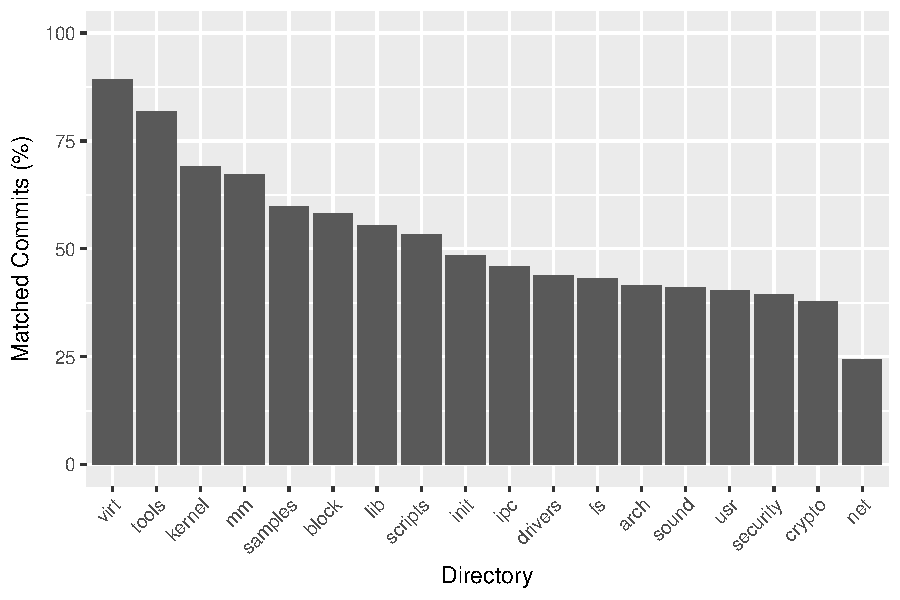
\includegraphics[scale=.6]{plots/matched_commits_dir}
  \caption{Percentage of matched commits in Linux subdirectories, from 2009 to the time of writing this paper.}
  \label{fig:matches_dir}
\end{figure}



%patch-based: \citep{msr13jojo,jiang14}
%actually, we're leveraging heuristic also mentioned by Jojo~\citep{jiang14} because nowadays it is standard practice <=> only from 2013 on? use only those in test

%\subsection{Formula for Historical Expertise}
%\label{sec:form-hist-expert}
%
%\begin{itemize}
%\item maybe, if too long to put in RQ2's approach
%\end{itemize}



\section{Case Study Results}
\label{sec:case-study-results}

This section discusses for each research question its motivation, specific approach and results.

\subsection*{RQ1. \rqone}
\label{sec:rq1.-how-does}

{\bf Motivation:} 

Open source software maintainers are responsible for the health of their subsystem. For example, each Linux kernel maintainer % ensures the healthy evolution of the Linux kernel
manages the changes proposed by developers to the subsystem they are responsible for, and shepherd those changes upstream towards the Git repository of Linus Torvalds (i.e., the official Linux kernel repository). Hence, their presence is vital to the kernel community.

Unfortunately, due to the unpredictable nature of life in general and open source software development in particular~\citep{Wu,Zhou}, maintainers, for various reasons, one day will be forced to give up their responsibilities. In most cases, this means that another developer will have to take over the responsibility of maintainer.

Hence, this research question aims to analyze how often maintainership changes in kernel development. Furthermore, we are interested in understanding how much of the code base of official releases is ``owned'' by the subsystem maintainers, i.e., was originally developed by a maintainer. Since ``git blame'' is a popular means for finding experts~\citep{Rahman-2011}, our results will help us understand to what extent such a measure is reliable to measure expertise.%  This allows to , as well as whether the workload of kernel developers also decreases over time \bram{if Zhou already found this, why are we doing it again? or is \texttt{legacy} measuring something else? if so, what is link with Zhou et al.'s work?}. \bram{did not get an answer about this, so removing it}% We investigate whether this decline in monthly workload and the decline in LOC footprint result in a loss of expertise.

{\bf Approach:}

To confirm the presence of changes in maintainership during the evolution of the Linux kernel, we analyzed the maintainers recorded in the \texttt{MAINTAINERS} file of releases \textit{v3.5} to \textit{v4.11} to identify how often maintainers (dis)appeared. % We compare the list of maintainers for each subsystem listed in the \texttt{MAINTAINERS} files contained in both releases of the linux kernel and count the number of subsystems where changes occured.
Furthermore, for each studied release, we measure and plot these maintainers' \texttt{legacy}, which corresponds to the number of surviving code lines of a maintainer, as given by ``git blame''. %understand the evolution of the LOC footprint of maintainer across time, we look at the "blame count" of each maintainer in each main linux release of the past 5 years. The blame count only contains the \textit{visible} lines of code associated with the maintainer in the files belonging to their subsystem.
We then validated the statistical significance of the change in \texttt{legacy} distribution between the first and last analyzed release using a Wilcoxon paired test. % between the \texttt{legacy} distribution of maintainers active in the studied period of .  
% list1=[across all maintainers of their \%lines owned in earliest release for given subsystem]
% list2=[same, in final release for which we have data for that person]
In case of a significant test result, we also provide the Cliff Delta effect size ((Cite Romano stats paper)). An effect size smaller than 0.147 is deemed a ``negligible'' difference, smaller than 0.33 a ``small'' difference, smaller than 0.474 a ``medium'' difference and otherwise a ``large'' difference.


\begin{figure}[t]
  \centering
  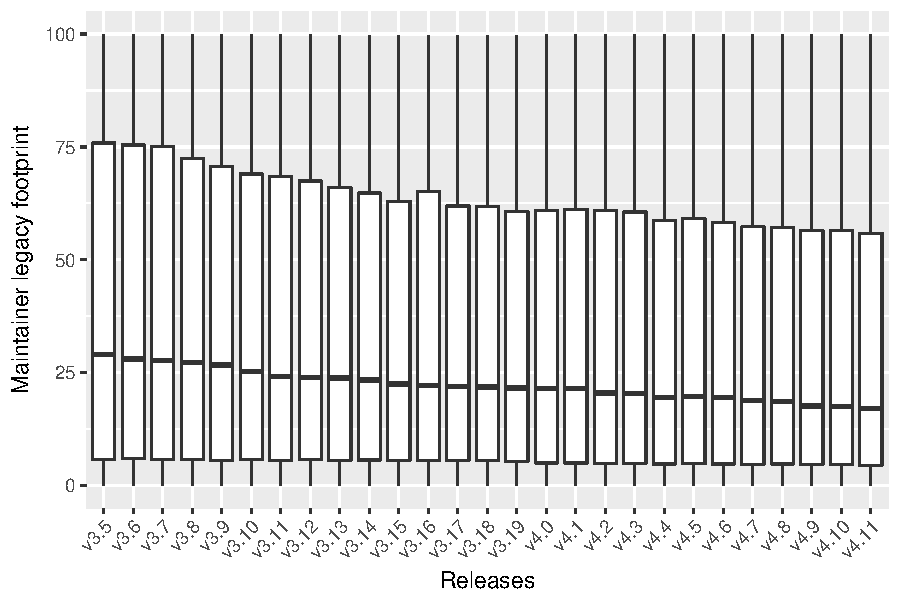
\includegraphics[scale=.6]{plots/RQ1_median_LOC}
  \caption{Median maintainer \texttt{legacy} across releases.}
  \label{fig:RQ1_temp}
\end{figure}

{\bf Results:}

\textbf{23\% of the studied subsystems saw changes in maintainership over the last 5 years.} Out of the 734 subsystems studied for RQ1, we counted 168 subsystems that experienced some sort of maintainership change. We counted 100 maintainer arrivals, 63 departures, and 88 replacements. These numbers confirm that maintainership change is common, even in mature open source systems like the Linux kernel. Furthermore, the median percentage of developers who are maintainers in the analyzed subsystems is 0.50\% (mean of 0.90\%), indicating that it is not straightforward to guess the next maintainer. These observations strengthen our case for more advanced expertise measures.

%\bram{do we have median plots now?}
\textbf{The median maintainer \texttt{legacy} significantly decreases over time.} \autoref{fig:RQ1_temp} shows the evolution of the median percentage of maintainer \texttt{legacy} across all subsystems in each studied release. The plot shows a clear, steady decrease of this measure across releases in terms of median and variance. We confirm the significance of this decrease with a Wilcoxon paired test ($\alpha=0.01$) between the first and last studied version, which yields a p-value of 2.2e-16.% We conclude that there is a significant decrease in LOC footprint during the observed period.


%\bram{no link at all with Zhou et al.'s work, it seems, as they? do we have better motivation? if not, leave out \autoref{fig:RQ1_temp}?}
Although the Cliff Delta value of 0.07 indicates only a negligible difference, this decreasing trend suggests that, if one limits the measure of expertise to the amount of surviving code originally authored by a maintainer, as was done by earlier work~\citep{Rahman-2011}, the expertise of maintainers globally seems to be decreasing over time. The next two research questions evaluate the use of a wider range of activity measures, across a range of releases, to obtain a more accurate measure of expertise.

% \bram{no link at all with Zhou et al.'s work, it seems, as they? do we have better motivation? if not, leave out \autoref{fig:RQ1_temp}?}

%\bram{still don't understand the link with Zhou et al., so leaving it out} This finding mirrors those of Zhou et al.~\citep{Zhou-fse}, who have shown that the workload of Linux kernel maintainers over time is decreasing. This workload was defined by the number of files a maintainer is responsible for, the number of commits to those files authored by other authors, and the number of authors interacting with the maintainer. Not only is the total workload not evenly spread out across all maintainers, their monthly workload is decreasing as well.


%The     According to state of the art expretise metrics, this decline in LOC footprint should translate in a decline in expertise.
% \begin{itemize}
%   \item Number of subsystems experiencing maintainer changes over studied period: 168 / 734 = 22.8\%.
%   \item Wilcoxon text between first and last LOC footprint: paired: 2.2e-16 / without paired = TRUE : 0.02653
% \end{itemize}
%Wilcoxon test (paired!) between list1 and list2 => alpha value of 0.01
% scatterplot or hexbinplot plot(list1,list2) 

% \bram{I think we are also missing boxplots saying, for each release, the percentage of subsystem contributors that is maintainer; this is important to indicate how hard it is to find a maintainer, since a subsystem with only 2 contributors is super-simple to identify maintainers for} \alex{I just computed all the maintainer/developer ratios: median is 0.5 percent (in the 78 filtered subsystems), so the boxplot doesn't look very good.}\bram{is this median across all releases and subsystems?}

% I found the evolution of the median percentage of maintainers in their subsystem across all releases:  median of 0.5% is for all subsystems in the current release; mean is 0.9%

% release,percentage(%)
% 22,0.58170995671
% 21,0.534046345811
% 20,0.576080667824
% 19,0.583783049927
% 18,0.584750523467
% 17,0.597305919887
% 16,0.552486187845
% 15,0.574712643678
% 14,0.614125834666
% 13,0.6269377183
% 12,0.639506374632
% 11,0.646488699503
% 10,0.661158831115
% 9,0.694578429481
% 8,0.715749039693
% 7,0.739434694658
% 6,0.757586627448
% 5,0.784361975362
% 4,0.785857650146
% 3,0.82305920607
% 2,0.82372881356
% 1,0.85231394168


\subsection*{RQ2. \rqtwo}
\label{sec:rq2.-does-current}

{\bf Motivation:}

% important => currently state-of-the-art is based on code activity => evaluation shows it is far from perfect, so we check and see that priorities of people have changed

Prior work on expertise measures~\citep{Anvik-2006, Bhattacharya, McDonald, Minto-2007, mockus02} primarily are based on code activity, which can be defined in terms of \texttt{legacy} and \texttt{committed}% number of changes added to the source code (Commits)
. As motivated in \autoref{sec:expertise-formula}, we believe that these two metrics do not capture the full breadth of contributor expertise activities. Indeed, the results in RQ1 indicate that the \texttt{legacy} of long-standing maintainers crumbles over time. Unless one assumes that this reflects a real drop in expertise over time, the only explanation is that existing experts reorient their focus to other activities, such as code review and email communication. Hence, this research question evaluates whether considering such additional activities is able to improve the identification of experts.%Other facets of software development are not reflected by those metrics. Important development activities such as code reviews and upstream committing are not portayed by lines of code and commit authors.

{\bf Approach:}

% To validate this technique, we need a proven expertise indicator. This indicator would help us confirm wether or not an expertise measuring approach is accurate. In the case of the linux kernel, we believe maintainership is a good expertise indicator. Maintainers are responsible of the health and sustainability of their subsystem. Developers often reached this position by demonstrating a long record of involvement in subsystem discussion and contributions. In other terms, they are regarded as experts in their subsystems by the community. 

% With the assumption that maintainers are experts in their subsystems, we can validate the expertise measured by our different approaches by comparing maintainership and high expertise score. 

% The naive expertise calculation requires two different data points. On one hand, we extract a list of subsystems as well as their current maintainers and the list of files contained in the subsystem. On the other hand, we create a line of code count for each developer.

% Git blame makes it easy to count each developer's line of code count. We execute git blame on each files in the linux source code. For each of those files, we created a ranking of developers in terms of lines of code. With the acquired subsystem file tree, we are capable of aggregating the line of code developer ranking to the subsystem level. 

% Furthermore, we are able to apply the same technique to aggregate the other metrics to the subsystem level. 

To validate the ability of the measures in \autoref{tab:metlin} to explain expertise, we evaluate how well the $footprint_j(\mathbb{A})$ measure involving those measures is able to identify the maintainers of Linux kernel subsystems. Those maintainers are the experts listed in the \texttt{MAINTAINERS} file of a kernel release.

For a given release and subsystem, %different heuristics dicussed in section \ref{sec:contribution-footprint} in term of ability to detect experts, we look for the presence of maintainers and their position in their subsystem's different rankings. 
%We assume that maintainers have more experience in \textit{their} subsystem than other developers active in this subsystem. Therefore,
we should find the maintainers in the top positions when ranked based on footprint values. The combination of activity measures $\mathbb{A}$ that is able to systematically yield the correct maintainers across subsystems and releases could be assumed to be a better indication of expertise. 

In particular, we calculate two performance metrics:
\begin{description}
\item[$POS_N$] \underline{P}ercentage \underline{O}f \underline{S}ubsystems for which at least one maintainer was ranked in the top N expert candidates
\item[$POM_N$] \underline{P}ercentage \underline{O}f \underline{M}aintainers in the {\em whole} project who were ranked in the top N expert candidates for their subsystem
\end{description}

For these performance metrics, N is a threshold that can be varied. Our case study uses thresholds ranging from 1 to 5. It is important to note that, if the number of maintainers of a subsystem is larger than N, $POM_N$ could be penalized. To avoid this, we slightly changed the definition of $POM_N$ to be calculated only for the maintainers of all subsystems with at most N maintainers, instead of for all maintainers of the whole project. For example, $POM_1$ measures the percentage of top-recommended maintainers of subsystems with at most 1 maintainer.%having said that, how do we explain that for top-N it says out of all projects with at most N maintainers, what is percentage of them in top-N?

To structure our analysis, we analyzed the performance of expertise models involving only one metric of \autoref{tab:metlin}, then analyzed models involving all combinations of \texttt{legacy} with one of the other 4 measures, and finally one model with all measures combined. We focus explicitly on models involving \texttt{legacy} because it is a commonly used measure ~\citep{Rahman-2011}, and hence we use its performance as baseline. %We excluded the 20 other combinations because we aim to analyze the impact of the different activities combined with \texttt{legacy}. \bram{basically: we chose A and B, because we chose A ...}
% \bram{why?}\alex{Too complicated to compute for such marginal returns?} \bram{no, we wanted to study the impact of different groups of metrics, i.e., blame, then commit info, then review info}

Since, for a given release, there is one $POS_N$ value and one $POM_N$ value, we calculate these metrics for each release, then study their distribution across the analyzed releases using boxplots. % Second, we also measure for each subsystem whether the top N ranking finds at least one of the subsystem's maintainers (since finding one maintainer is enough for someone trying to ask a question).%We establish thresholds of a maximum ranking position to validate wether a metric or combination of metrics is a good expertise indicator. In other words
\autoref{fig:rq2_1} and \autoref{fig:rq2_3} show for each analyzed $\mathbb{A}$ % the performance of each studied metric and combination of metrics for
the distributions of $POS_N$ for N=1 and N=3, respectively, across the 22 studied Linux releases, while \autoref{fig:rq2_1_many} and \autoref{fig:rq2_3_many} the distributions of $POM_N$ for N=1 and N=3, respectively. % the proportion of \textit{subsystems} with at least one correctly identified within the top N footprint values of the subsystems, across the 22 studied Linux releases. 
We only show the plots for N=1 and N=3, as for higher values of N the plots remain more or less stable.
% TODO: stress other approaches used by other papers as baseline (legacy, committed)
% TODO: what is distribution of footprint values per subsystem? 1 clear winner?


% We track the following metrics:
% \begin{itemize}
% \item Number of LOC 
% \item Number of commits as author
% \item Number of commits as committer
% \item Number of review emails/reviewed patches
% \item Number of Commit message attributions
% \end{itemize}


 
%\begin{itemize}
%\item git blame
%\item currently most active developers: number of commits since last release (total since beginning not practical, since those people away) <=> not that easy to calculate yourself (until Jonathan Corbet releases his report) + only new contributions
%\end{itemize}



\begin{figure*}[t]
  \centering
  \begin{minipage}[b]{\columnwidth}
    \centering
    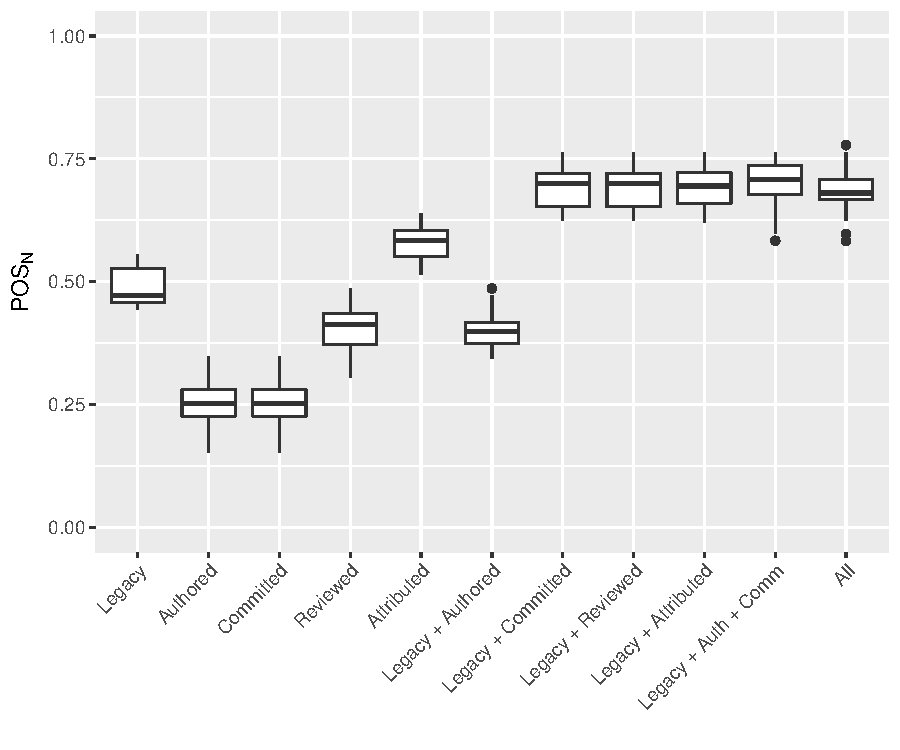
\includegraphics[scale=.55]{plots/RQ2_metrics_N1_one_maint}
    \caption{Distribution of $POS_N$ for each combination of activity measures, for ranking threshold N = 1. }
    \label{fig:rq2_1}
  \end{minipage}
  % \hfill
  \begin{minipage}[b]{\columnwidth}
    \centering
    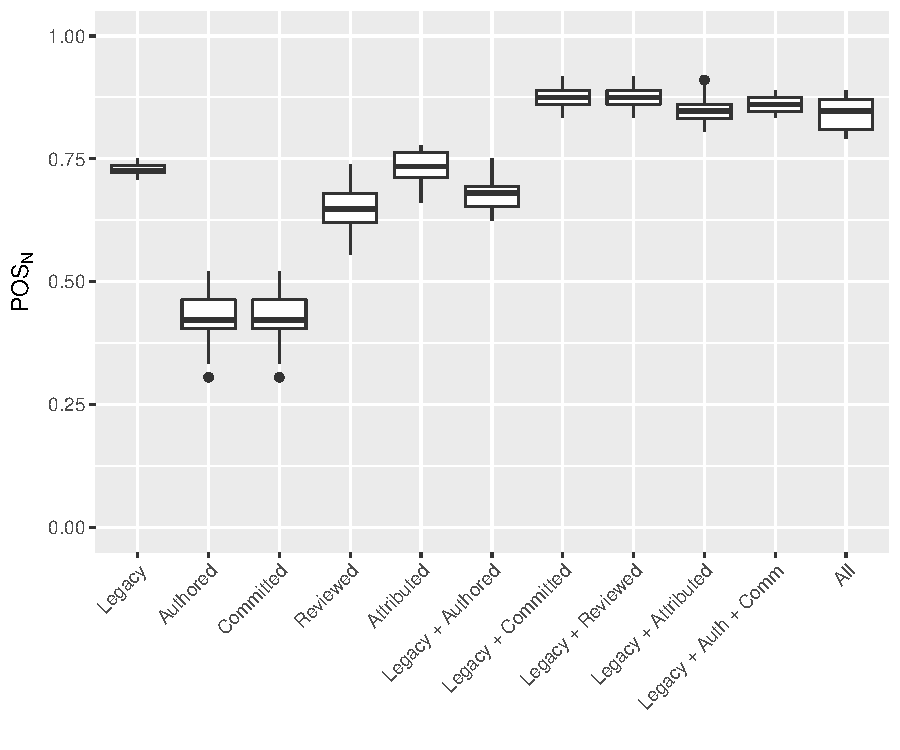
\includegraphics[scale=.55]{plots/RQ2_metrics_N3_one_maint}
    \caption{Distribution of $POS_N$ for each combination of activity measures, for ranking threshold N = 3. }
    \label{fig:rq2_3}
  \end{minipage}
\end{figure*}

\begin{figure*}[t]
  \centering
  \begin{minipage}[b]{\columnwidth}
    \centering
    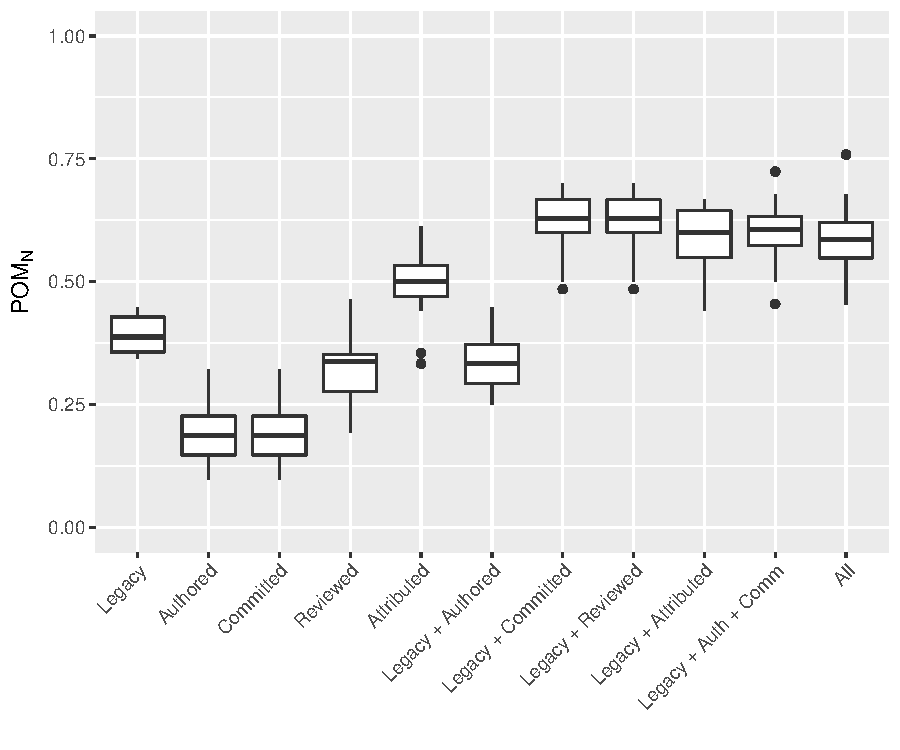
\includegraphics[scale=.55]{plots/RQ2_metrics_N1_many_maint}
    \caption{Distribution of $POM_N$ for each combination of activity measures, for ranking threshold N = 1. These boxplots only consider subsystems with at most 1 maintainer.}
    \label{fig:rq2_1_many}
  \end{minipage}
  % \hfill
  \begin{minipage}[b]{\columnwidth}
    \centering
    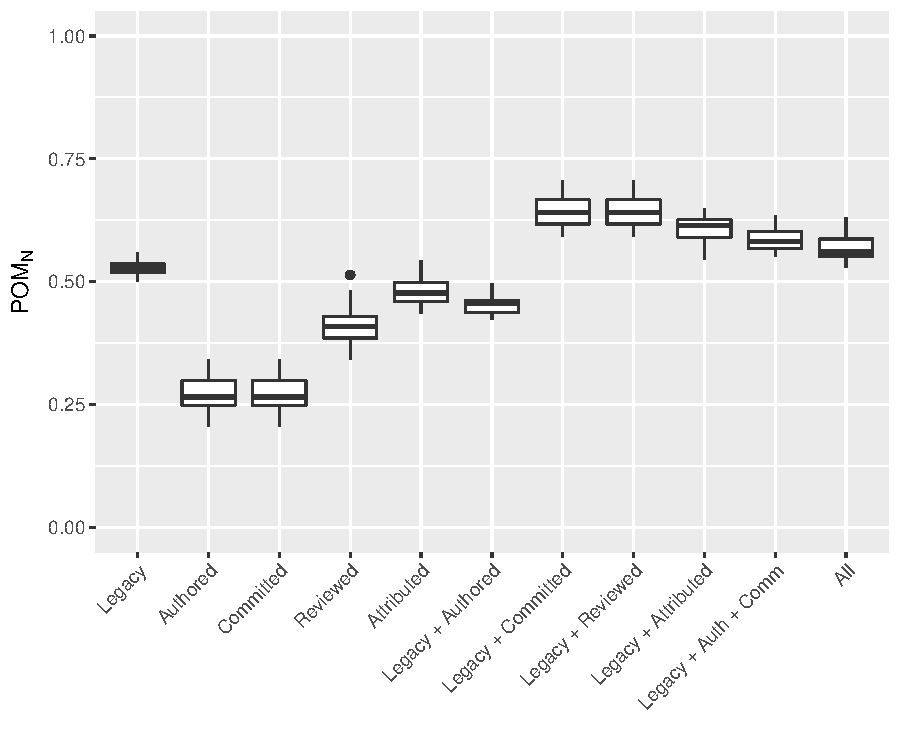
\includegraphics[scale=.55]{plots/RQ2_metrics_N3_many_maint}
    \caption{Distribution of $POM_N$ for each combination of activity measures, for ranking threshold N = 3. These boxplots only consider subsystems with at most 3 maintainers.}
    \label{fig:rq2_3_many}
  \end{minipage}
\end{figure*}



{\bf Results:}

\begin{table}[t]
\centering
 \begin{tabular}{c c c c c c c} 
 Type & Measure & N = 1 & N = 3 \\
 \hline
  $POS_N$ & P-value       & 4.27e-05 &  4.28e-05  \\
  $POS_N$ & Cliff's delta & 0.99    & 1.0     \\
  $POM_N$ & P-value       & 4.27e-05 & 4.77e-07  \\
  $POM_N$ & Cliff's delta & 0.84    & 1.0     \\
\end{tabular}
\caption{P-values and Cliff's delta values for the Wilcoxon paired tests ($\alpha=0.01$) between \texttt{attributed} and \texttt{legacy + committed} for ranking thresholds N=1 and N=3 and for $POS_N$ and $POM_N$.}
\label{table:rq2_wilc_att_loc_cc}
\end{table}

% After filtering out inactive and small subsystems, we are left with a subset of 78 subsystems. We ran the experiments with rankings thresholds from 1 to 5 on 22 different releases of the linux kernel (v3.8 to v4.11). 

\textbf{\texttt{attributed} is the only single-measure model able to keep up with the multi-measure models.} 

The results in \autoref{fig:rq2_1} and \autoref{fig:rq2_1_many} indicate that the first two individual measures, i.e., \texttt{legacy} and \texttt{authored}, are bad indicators of expertise compared to the other studied metrics. For example, in \autoref{fig:rq2_1}, \texttt{legacy} only reaches a median $POS_N$ value of 47.22\%, while \texttt{attributed} reaches a median $POS_N$ percentage of 58.4\%.

\textbf{The models combining \texttt{legacy} with \texttt{committed}, \texttt{attributed} and/or \texttt{reviewed} perform the best.} \autoref{fig:rq2_1} shows indeed how only these four models read median percentages of 69.9\%, while the other multi-measure models, especially the one involving only \texttt{legacy} and \texttt{authored}, are not able to outperform the best individual measure models. %The model becomes increasingly accurate when we build rankings based on a combination of metrics. These combinations allow for a wider representation of the different activities that make up linux kernel development.

These findings confirm the intuition that maintainers shifted focus from doing development (\texttt{authored}) themselves to mentoring others by controlling access to their subsystem's Git repository through committing and/or reviewing. As such, an expertise model only involving their own development (i.e., \texttt{legacy} and \texttt{authored}) is unable to explain the current kernel maintainers' expertise. In other words, modern expertise models should take into account the time spent reviewing code and pushing changes upstream.% should be accounted for in the implementation of an expertise measure.

% Combining different, unrelated metrics allows the model to compensate a decrease of one data point by an increase of another. For instance, a maintainer's decline in LOC footprint could be explained by an increase in code review, which would prevent the maintainer to contribute as much code as he used to. 

\textbf{$POS_N$ increases to a median of 87.5\% for larger N, with multi-measure models outperforming single-measure models by at least 17\%.} Comparing \autoref{fig:rq2_3} to \autoref{fig:rq2_1} shows how the top multi-measure models for N=1 are able to increase their distance compared to even the best single-measure models (\texttt{attributed}). This, compared with a change in best performing single-measure models, indicates that a larger diversity in activity measures enables better identification of the two additional candidate maintainers. Indeed, by considering top performing contributors across a wider range of activities, there is a larger chance at least one real maintainer is found. Although the percentages of \autoref{fig:rq2_1_many} and \autoref{fig:rq2_3_many} cannot be compared directly to each other (cf. modified definition of $POM_N$), \autoref{fig:rq2_3_many} (for $POM_N$) shows a similar ranking of models as \autoref{fig:rq2_1} (for $POS_N$), confirming the findings for $POS_N$.

\autoref{table:rq2_wilc_att_loc_cc} shows the p-value and effect size of the Wilcoxon test between \texttt{attributed} and \texttt{legacy + committed} for figures \ref{fig:rq2_1}, \ref{fig:rq2_3}, \ref{fig:rq2_1_many}, and \ref{fig:rq2_3_many}. Each effect size being close to 1, we notice a \textbf{large} performance increase between \texttt{attributed} and \texttt{legacy + committed}.

Interesting to note is that, across all analyzed releases, the boxplots show a remarkable small variance, especially for N=3. Although this is partially due to the fact that less than 25\% of the subsystems saw at least one maintainer change, it also indicates that our measures are stable across changes in the 5 activity measures used.%A metric combination that returns a higher than average accuracy is \textit{Lines of Code(LOC) + Commits Committer.} This proves that the decline in lines of code footprint does not indicate \textit{expertise erosion}, but rather, a shift in priorities between writting code and upstream committing??. 
% Maintainers are able to keep their level of expertise by staying involved 

%\begin{itemize}
%\item existing work looks at how much code still left in current version of code or how many commits done in latest release (cite papers): how does this expertise evolve across releases for each maintainer? => we will see drop
%\item why? they perform less commits, so their footprint on code is dropping + moving towards reviewing instead making commits themselves
%\item their code is eroding
%\end{itemize}



\subsection*{RQ3. \rqthree}
\label{sec:rq3.-does-historical}

{\bf Motivation:} 

% priorities seem to shift => add historical expertise + expertise in different activities (in particular code review, although there are other things we do not measure)
The metrics analyzed in RQ2 reveal that traditional expertise metrics based solely on a contributor's own development productivity are not well suited to identify maintainers. Expertise models exploiting only the information available for the release under study, are able to obtain median $POS_N$ performance of up to 75\% (N=1) and 90\% (N=3).%   first dimOther metrics, such as number of commits as a committer and number of commit message attributions are better indicators of maintainership. We believe this is due to a shift from development to reviewing activities. 

However, % the limitation of $footprint_j(\mathbb{A})$ is that it only accounts for the data found in the current release of the kernel. We
we believe that adding a historical dimension considering also the activity in the last R releases would assist the model in two ways. On the one hand, long standing kernel developers' contributions should carry more weight than newcomers' contributions. On the other hand, analyzing data on multiple releases would control for cases where contributors' productivity was lower due to a variety of reasons, such as illness, vacation or work on other projects.
%For these reasons, this research question evaluates the ability of the history-awaware $footprint_j^R(\mathbb{A})$ to explain expertise.
% The metrics used in RQ2 reveals a large difference between the existing measure of expertise and the official list of maintainers. We believe that this is due to the narrowness of the observed data points. As discovered in RQ1, maintainers have to focus their time on not only contributing to their subsystems, but also in reviewing the often large amount of patches being sent by other developers/contributors. We believe that this sort of activities should be accounted for in the implementation of an expertise measure. 





% looks at the number of code contributions for the latest observed Linux release (4.11). 

%previous RQ shows big gap between existing measures of expertise and official list of maintainers => reason: they ignore the erosion of expertise over time, where physical code presence slowly turns into more management-level activities => expertise does not vanish, just another form



{\bf Approach:}

%We tracked the different subsystems over a five year period. This allowed us to aggregate contributions, commits, and number of patches reviewed during the last 27 releases of the Linux kernel.
For each studied kernel release, we calculated $footprint_j^R(\mathbb{A})$ for R=4, since this covers a time span of 60 to 70 days. For example, when looking at experts in release \textit{v4.11}, we need to take into account data found for releases \textit{v4.7, v4.8, v4.9, v4.10, and v4.11}. We repeat such analysis for each of the 22 releases. In this paper, we use linearly decaying weights $W_i$ to combine the individual $footprint_j(\mathbb{A})$ values across the five considered releases, since this scheme is less extreme than the exponential and logarithmic ones.

Similar to RQ2, we then use the footprint values to create, for each subsystem and release, a ranking of all contributors active in the five considered releases% present in the last five release of the subsystem. We repeat this step for each studied subsystem and then for the last 22 releases
. We also use the same performance metrics as for RQ2, which allows us to compare the results of RQ3 to those of RQ2 to validate % .
% We can now apply the technique described in the approach of RQ2, and verify 
whether the historical dimension improves the model.

To save space, and since we found that, similar to RQ2, the combination of \texttt{legacy} and \texttt{committed} performs the best, we only show the results for this model (the rest of the data will be made available after the double-blind review). In particular, % maybe need exponentially decaying weights, where past counts, but newer stuff has higher weight
\autoref{fig:rq3_curr} and \autoref{fig:rq3_hist} show the $POS_N$ performance of the combined \texttt{legacy}+\texttt{committed} model without and with the history dimension, for ranking thresholds N ranging from 1 to 5. \autoref{fig:rq3_curr_many} and \autoref{fig:rq3_hist_many} show the corresponding $POM_N$ results.%\bram{also, did you double-check that this combined model is still the best one?} \alex{It is the best one, but it is already really good for the current percpective, so the performance increase is not as noticable when using historical. See table 3.} 

\autoref{table:rq3_wilc_loc_cc} contains the results of Wilcoxon paired tests between the $POS_N$ values without and with history, for each N, and (similarly) between the $POM_N$ values without and with history, for each N. For each test, we also provide the Cliff Delta effect size(((cite romano))).% An effect size smaller than 0.147 is deemed ``negligible'', smaller than 0.33 ``small'', smaller than 0.474 ``medium'' and otherwise ``large''.

% To create rankings in a similar fashion as RQ2, we assign previous release data to linearly decaying weights. The data collected in \textit{v4.7} will carry less weight than the data found in \textit{v4.8}, as developers are less likely to lose experience acquired more recently \citep{Rigby}. 

% For each developer found in each tracked subsystem, we compute and weight the different metrics for the past 4 releases. For example: 

% \[
% \Big[M_{t-4}, M_{t-3}, M_{t-2}, M_{t-1}, M_{t} \Big]
% \]

% Where $M_t$ = the metrics collected for a developer in a given subsystem for release t. 

% \[
% W = \Big[0.2, 0.4, 0.6, 0.8, 1.0 \Big]
% \]

% \[
% Expertise Index = \sum_{t=1}^{5} M_{t} W_{t}
% \]

% ((( TODO: Cleanup equation)))


% need to filter data set based on number of maintainers, maybe their percentage of changed code/commits across time, ... => makes it more interesting for evaluation (harder to determine right answer)

% also need enough activity in subsystems that we study here, for example large enough percentage of releases in which they made at least one commit, or large enough average number of commits per release => maybe already do this at end of preliminary analysis?

\begin{figure*}[t]
  \centering
  \begin{minipage}[b]{\columnwidth}
    \centering
    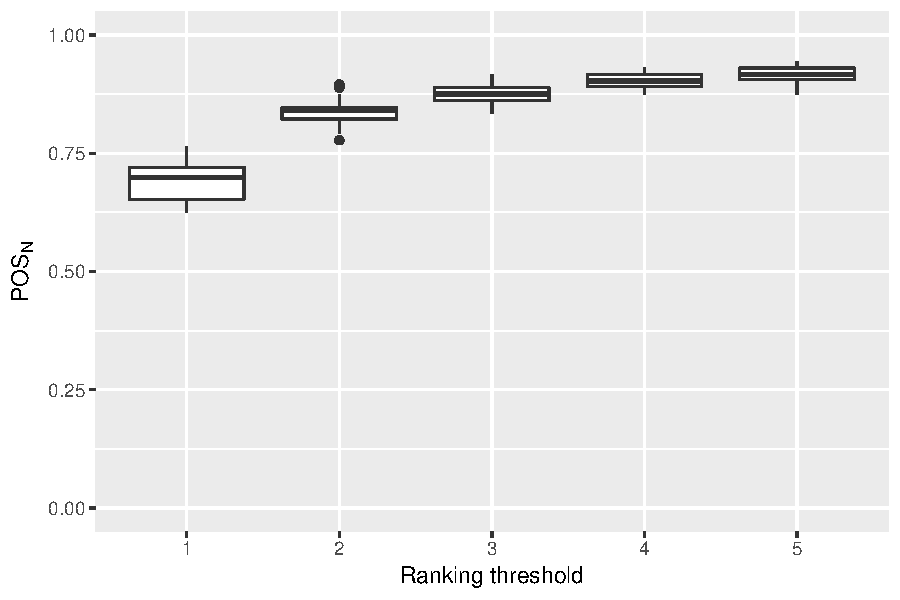
\includegraphics[scale=.6]{plots/RQ3_curr}
    \caption{Distribution of $POS_N$ for the combined \texttt{legacy}+\texttt{committed} model (\textbf{without} history dimension), for different N.}
    \label{fig:rq3_curr}
  \end{minipage}
  % \hfill
  \begin{minipage}[b]{\columnwidth}
    \centering
    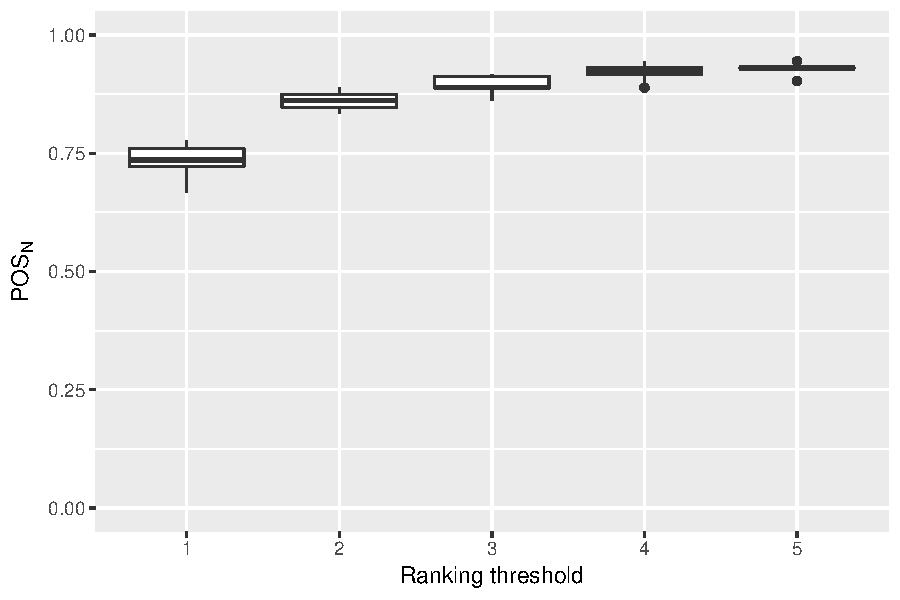
\includegraphics[scale=.6]{plots/RQ3_hist}
    \caption{Distribution of $POS_N$ for the combined \texttt{legacy}+\texttt{committed} model (\textbf{with} history dimension), for different N.}
    \label{fig:rq3_hist}
  \end{minipage}
\end{figure*}

\begin{figure*}[t]
  \centering
  \begin{minipage}[b]{\columnwidth}
    \centering
    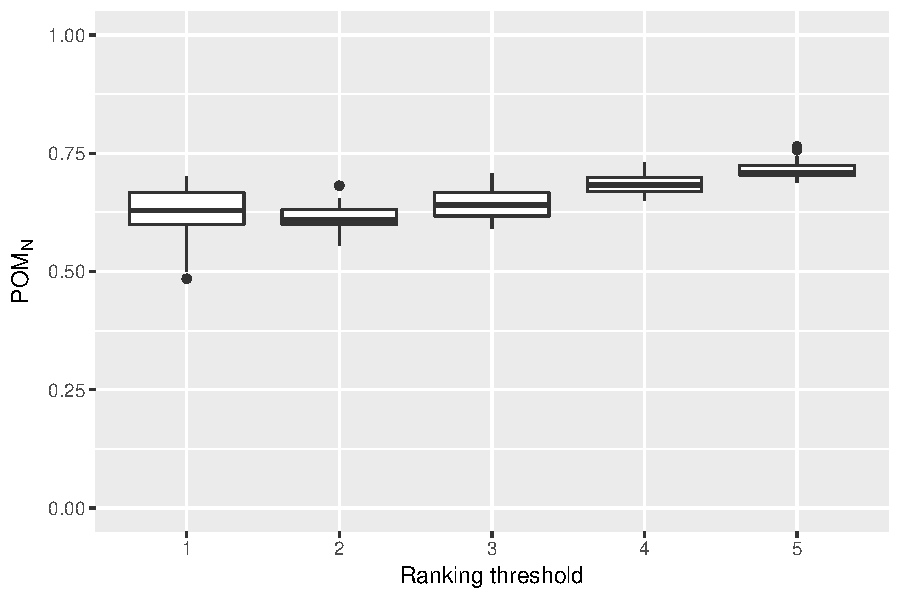
\includegraphics[scale=.6]{plots/RQ3_curr_many}
    \caption{Distribution of $POM_N$ for the combined \texttt{legacy}+\texttt{committed} model (\textbf{without} history dimension), for different N. For each N, the boxplot only considers subsystems with at most N maintainers.}
    \label{fig:rq3_curr_many}
  \end{minipage}
  % \hfill
  \begin{minipage}[b]{\columnwidth}
    \centering
    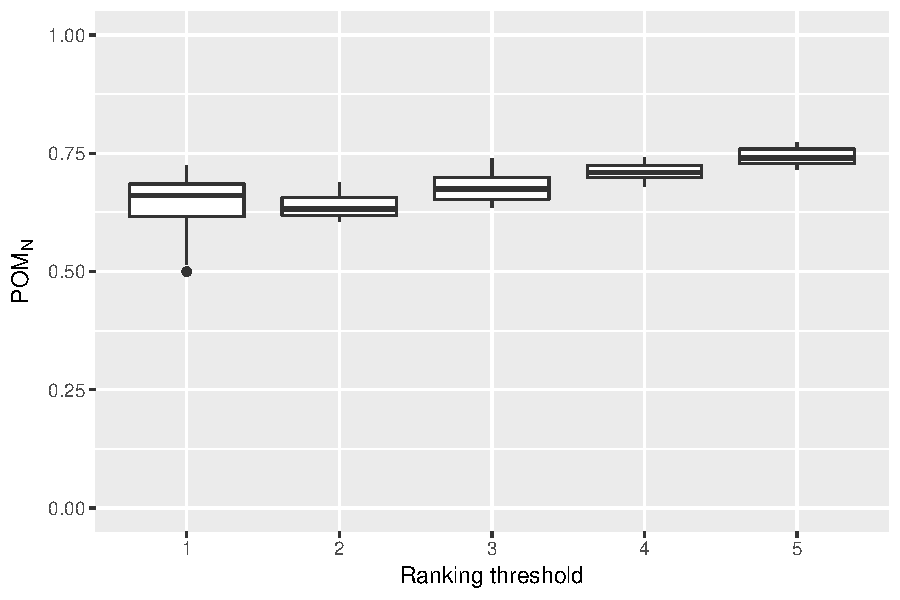
\includegraphics[scale=.6]{plots/RQ3_hist_many}
    \caption{Distribution of $POM_N$ for the combined \texttt{legacy}+\texttt{committed} model (\textbf{with} history dimension), for different N. For each N, the boxplot only considers subsystems with at most N maintainers.}
    \label{fig:rq3_hist_many}
  \end{minipage}
\end{figure*}



% \begin{table}[t]
%  \begin{tabular}{c c c c c c} 
%  Threshold N & 1 & 2 & 3 & 4 & 5 \\
%  \hline
%  P-value & 6.7e-05 & 5.7e-05 & 9.3e-05 & 2.1e-04 & 1.2e-04 \\
%  Cliff's delta & 0.6632 & 0.9442 & 0.7706 & 0.6384 & 0.6198
% \end{tabular}
% \caption{Cliff's delta and  p-values for the Wilcoxon paired tests between the performance results for the combined \texttt{legacy}/\texttt{authored}/\texttt{committed}, for ranking thresholds N=1 to N=5.}
% \label{table:rq3_wilc}
% \end{table}

\begin{table}[t]
 \begin{tabular}{c c c c c c c} 
Fig. & Measure & 1 & 2 & 3 & 4 & 5 \\
 \hline
\ref{fig:rq3_curr}/\ref{fig:rq3_hist} & P-value & 1.12e-4 & 8.76e-3 & 1.15e-2 & 1.57e-3 & 7.70e-4 \\
% \ref{fig:rq3_curr}/\ref{fig:rq3_hist}& Cliff's delta & 0.62 & 0.50 & 0.43 & 0.55 & 0.51 \\
      \ref{fig:rq3_curr}/\ref{fig:rq3_hist}& Cliff's delta & 0.62 & 0.50 & - & 0.55 & 0.51 \\
\ref{fig:rq3_curr_many}/\ref{fig:rq3_hist_many} &  P-value & 1.27e-2 & 4.63e-3 & 5.13e-4 & 1.57e-5 & 1.88e-4 \\
% \ref{fig:rq3_curr_many}/\ref{fig:rq3_hist_many}& Cliff's delta & 0.25 & 0.46 & 0.56 & 0.66 & 0.69 \\
   \ref{fig:rq3_curr_many}/\ref{fig:rq3_hist_many}& Cliff's delta & - & 0.46 & 0.56 & 0.66 & 0.69 \\
\end{tabular}
\caption{P-values and Cliff's delta values for the Wilcoxon paired tests ($\alpha=0.01$) between the $POS_N$ results of \autoref{fig:rq3_curr} and \autoref{fig:rq3_hist}, and of \autoref{fig:rq3_curr_many} and \autoref{fig:rq3_hist_many}, for ranking thresholds N=1 to N=5. A Cliff delta ``-'' indicates a non-significant test result, with p-value$>\alpha$}
\label{table:rq3_wilc_loc_cc}
\end{table}


% \begin{table}[t]
%  \begin{tabular}{c c c c c c} 
%  Threshold N & 1 & 2 & 3 & 4 & 5 \\
%  \hline
%  P-value & 0.01267 & 0.004634 & 0.0005127 & 1.574e-05 & 0.0001884 \\
%  Cliff's delta & 0.2479339 & 0.4607438 & 0.5640496 & 0.6590909 & 0.6942149
% \end{tabular}
% \caption{Cliff's delta and  p-values for the Wilcoxon paired tests between the performance results for $POM_N$ for the combined \texttt{legacy}/\texttt{committed}, for ranking thresholds N=1 to N=5.}
% \label{table:rq3_wilc_plot9_10}
% \end{table}



{\bf Results:}

\textbf{The history-aware \texttt{legacy}+\texttt{committed} footprint models perform significantly better than the history-unaware models.} \autoref{fig:rq3_curr} and \autoref{fig:rq3_hist} show how, except for N=3, the median performance of the history-aware expertise measure improves upon the history-unaware measure. If one considers only the first recommendation of the measure, there is a median 73.6\% chance that at least one maintainer is identified for a history-aware expertise model compared to 69.9\% with the single-release model. This difference progressively decreases for higher N, which means that, for higher N, an expertise model considering \texttt{legacy}+\texttt{committed} on one release only is robust enough to assess expertise.

We find similar improvements for \autoref{fig:rq3_curr_many} and \autoref{fig:rq3_hist_many}, except that the improvements due to history increase for larger N (and for N=1 there is no significant improvement). This is clearly shown % The differences in performance between the models without and with history are significant, as is shown 
by the p-values and effect sizes of the Wilcoxon paired tests in \autoref{table:rq3_wilc_loc_cc} ($alpha=0.01$). As an effect size greater than 0.474 indicates a \textbf{large} increase in performance, we notice that 7 of the 8 significant differences have an effect size of at least 0.50. %Since all the resulting p-values are under 0.01, we safely reject $H_0$ and accept $H_1$. (((Revisit)))
%\bram{can we add more discussion here and in RQ2 about the subsystems for which performance was better/worse than other subsystems?}


\section{Discussion}
\label{sec:discussion}

\textbf{Threats to validity:}

Threats to external validity prevent generalization of empirical results to other contexts. In particular, due to the abundant volume of data and presence of an oracle for expertise, our empirical evaluation only focused on 22 releases of the Linux kernel project. Hence, the study should be expanded to cover not only more kernel releases, but also other open (and closed) source projects. Furthermore, we considered only 5 expertise measures for our footprint models. Other measures, such as those mentioned in \autoref{tab:met}, should be studied to understand their impact on expertise.
% \begin{itemize}
% \item only Linux kernel
% \item only 22 releases
% \item only 5 measures
% \end{itemize}

Threats to construct validity involve risks regarding the measures used in the empirical study. Of the five considered expertise measures, \texttt{reviewed} was the only one requiring noisy approximations. Except for cases where the email patch subject was identical to the Git commit message summary, there is a definite risk of false positive and false negative matches, as identified earlier by Jiang et al.~\citep{msr13jojo,jiang14}. This might explain the relatively weak performance of expertise models involving \texttt{reviewed}. However, no better alternatives exist for projects that use mailing lists for code review. Projects using web-based review environments like Gerrit do not have this issue, and will have perfect matching between commits and their reviews.
% construct:
% \begin{itemize}
% \item matching not perfect => sub-par performance of review-related metrics could be explained by this
% \end{itemize}

Finally, regarding threats to internal validity (i.e., confounding factors potentially explaining our findings), we mention the limited number of subsystems considered for RQ2 and RQ3. This number was the result of the data filtering in \autoref{sec:data-filtering} used to eliminate temporarily inactive subsystems. Furthermore, we used the \texttt{MAINTAINERS} file as oracle for expertise. Although this is the known reference in the Linux kernel community for finding the right maintainer to contact, this is a manually maintained text file that hence could contain inconsistencies (even though changes to it are peer-reviewed).

Finally, although maintainership is a form of expertise, there are other forms of expertise that our footprint models be indicators of that were not considered in our empirical study. As such, some of the false positive recommendations of our footprint rankings might actually be correct suggestions based on a different interpretation of expert, in which case our $POS_N$ and $POM_N$ results are lower bounds for the actual performance.
% internal:
% \begin{itemize}
% \item limited number of subsystems for RQ2 and RQ3 due to filtering
% \item using kernel maintainers as experts
% \end{itemize}


\textbf{Future work:}

Apart from addressing the threats to validity, other future work should consider different weights $w_i$ and $W_i$. The former weights consider different activities to be more relevant than others, while the latter weights would give more or less weights to older vs. newer releases. For example, comparison of exponential and logarithmic decaying weights to the linear decay used in our study could be interesting. Similarly, different values of $R$ for $footprint_j^R(\mathbb{A})$ should be evaluated.

%Deeper analysis of email reviews

%Additional activity measures, such as churn, regular email activity, etc.

%Manually identify experts who are not necessarily maintainers, and use them to further validate model

%future work: alternative approach would be to look at characteristics of experts and those becoming new maintainer, then explanatory model to find major characteristics (we instead did a constructionist approach)
Finally, whereas we used a top-down approach from expertise model to evaluation on an actual open source project, a bottom-up approach starting from the analysis of a project's or subsystem's maintainers before formulating expertise measures and models could provide complementary insights into different kinds expertise.

%other systems than Linux

%look at distribution of each measure, then transform in specific way in order to best separate values (e.g., also filtering too low values, ...)







% An example of a floating figure using the graphicx package.
% Note that \label must occur AFTER (or within) \caption.
% For figures, \caption should occur after the \includegraphics.
% Note that IEEEtran v1.7 and later has special internal code that
% is designed to preserve the operation of \label within \caption
% even when the captionsoff option is in effect. However, because
% of issues like this, it may be the safest practice to put all your
% \label just after \caption rather than within \caption{}.
%
% Reminder: the "draftcls" or "draftclsnofoot", not "draft", class
% option should be used if it is desired that the figures are to be
% displayed while in draft mode.
%
%\begin{figure}[!t]
%\centering
%\includegraphics[width=2.5in]{myfigure}
% where an .eps filename suffix will be assumed under latex, 
% and a .pdf suffix will be assumed for pdflatex; or what has been declared
% via \DeclareGraphicsExtensions.
%\caption{Simulation results for the network.}
%\label{fig_sim}
%\end{figure}

% Note that the IEEE typically puts floats only at the top, even when this
% results in a large percentage of a column being occupied by floats.


% An example of a double column floating figure using two subfigures.
% (The subfig.sty package must be loaded for this to work.)
% The subfigure \label commands are set within each subfloat command,
% and the \label for the overall figure must come after \caption.
% \hfil is used as a separator to get equal spacing.
% Watch out that the combined width of all the subfigures on a 
% line do not exceed the text width or a line break will occur.
%
%\begin{figure*}[!t]
%\centering
%\subfloat[Case I]{\includegraphics[width=2.5in]{box}%
%\label{fig_first_case}}
%\hfil
%\subfloat[Case II]{\includegraphics[width=2.5in]{box}%
%\label{fig_second_case}}
%\caption{Simulation results for the network.}
%\label{fig_sim}
%\end{figure*}
%
% Note that often IEEE papers with subfigures do not employ subfigure
% captions (using the optional argument to \subfloat[]), but instead will
% reference/describe all of them (a), (b), etc., within the main caption.
% Be aware that for subfig.sty to generate the (a), (b), etc., subfigure
% labels, the optional argument to \subfloat must be present. If a
% subcaption is not desired, just leave its contents blank,
% e.g., \subfloat[].


% An example of a floating table. Note that, for IEEE style tables, the
% \caption command should come BEFORE the table and, given that table
% captions serve much like titles, are usually capitalized except for words
% such as a, an, and, as, at, but, by, for, in, nor, of, on, or, the, to
% and up, which are usually not capitalized unless they are the first or
% last word of the caption. Table text will default to \footnotesize as
% the IEEE normally uses this smaller font for tables.
% The \label must come after \caption as always.
%
%\begin{table}[!t]
%% increase table row spacing, adjust to taste
%\renewcommand{\arraystretch}{1.3}
% if using array.sty, it might be a good idea to tweak the value of
% \extrarowheight as needed to properly center the text within the cells
%\caption{An Example of a Table}
%\label{table_example}
%\centering
%% Some packages, such as MDW tools, offer better commands for making tables
%% than the plain LaTeX2e tabular which is used here.
%\begin{tabular}{|c||c|}
%\hline
%One & Two\\
%\hline
%Three & Four\\
%\hline
%\end{tabular}
%\end{table}


% Note that the IEEE does not put floats in the very first column
% - or typically anywhere on the first page for that matter. Also,
% in-text middle ("here") positioning is typically not used, but it
% is allowed and encouraged for Computer Society conferences (but
% not Computer Society journals). Most IEEE journals/conferences use
% top floats exclusively. 
% Note that, LaTeX2e, unlike IEEE journals/conferences, places
% footnotes above bottom floats. This can be corrected via the
% \fnbelowfloat command of the stfloats package.




\section{Conclusion}

This paper argued about the need for expertise models considering a wide range of developer and other activities, and doing so across different snapshots of a project instead of just for one snapshot. Through an empirical study on 22 releases of the Linux kernel, we empirically showed how measures about an expert's own coding footprint (\texttt{legacy}) and her involvement in coordinating other project members (e.g., committing their commits and/or reviewing their code changes) significantly improves on coding-only expertise models. Furthermore, considering those measures across different releases significantly improved performance, with large effect size.

The simplest incarnation of our expertise model that software organizations should consider adopting involves (1) a developer's code \texttt{legacy} and number of changes \texttt{committed}, which are both readily obtainable from a Git log, calculated across (2) the last 5 releases. In future work, we will consider additional activity measures and empirically analyze other open source projects.


% The conclusion goes here.
% to really find who is expert, you need two things:
% \begin{itemize}
% \item different measures, not just blame and commit authors but also reviews, committers and commit message attributions
%   \item historical perspective
% \end{itemize}


% \bram{should talk about how good expertise measures are in general, the fact that mixing activities is a must, and that somehow review activities are less indicative, at least in the kernel community}

% RQ1:
% 23\% of the studied subsystems saw changes in maintainership over the last 5 years.
% The median maintainer \texttt{legacy} significantly decreases over time.

% RQ2:
% \texttt{attributed} is the only single-measure model able to keep up with the multi-measure models.
% The models combining \texttt{legacy} with \texttt{committed}, \texttt{attributed} and/or \texttt{reviewed} perform the best
% $POS_N$ increases to a median of 87.5\% for larger N, with multi-measure models outperforming single-measure models by at least 17\%.

% RQ3:
% The history-aware \texttt{legacy}+\texttt{committed} footprint models perform significantly better than the history-unaware models.





